\documentclass{beamer}
%\usepackage{BOONDOX-cal}

\definecolor{OliveGreen}{rgb}{0,0.6,0}

\usetheme[progressbar=frametitle]{metropolis}
\setbeamertemplate{frame numbering}[fraction]
\useoutertheme{metropolis}
\useinnertheme{metropolis}
\usefonttheme{metropolis}
\usecolortheme{spruce}
\setbeamercolor{background canvas}{bg=white}

\definecolor{mygreen}{rgb}{.125,.5,.25}
%\usecolortheme{crane}
\usecolortheme[named=mygreen]{structure}
\title{Named Entity Recognition}
\subtitle{Apply on Knowledg Graph and Sentiment Analysis}
\author{Phiphat Chomchit}
\institute{CMU}

\date{}
\begin{document}
	% Fill color in block
	\metroset{block=fill}
	\begin{frame}
		\titlepage
	\end{frame}

	\begin{frame}[t]{ Linguistic annotations}
		Linguistic annotations give you insights into a text’s grammatical structure.
		
		This includes the word types, like the parts of speech, and how the words are related to each other.
	\end{frame}

	\begin{frame}[t]{Tokenization}
		Segmenting text into words, punctuations marks etc.
		\begin{figure}
			\centering
			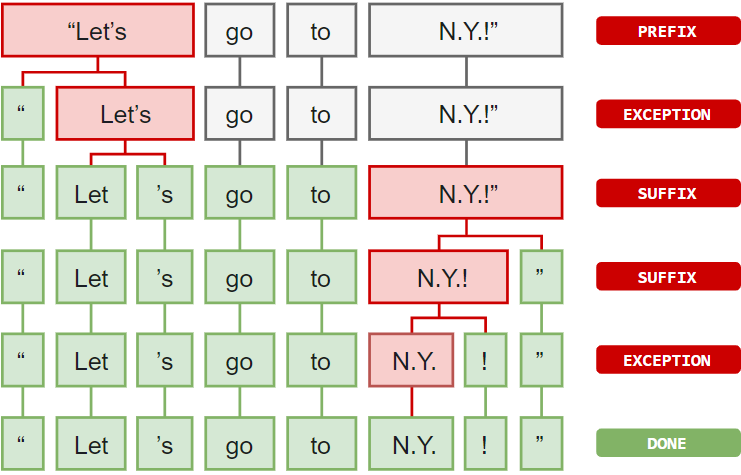
\includegraphics[scale=0.4]{token.png}
		\end{figure}
	\end{frame}

	\begin{frame}[t]{Part-Of-Speech (POS) Tagging}
		Part of speech or POS is a grammatical role that explains how a particular word is used in a sentence. There are eight parts of speech.
		\begin{enumerate}
			\item Noun
			\item Pronoun
			\item Adjective
			\item Verb
			\item Adverb
			\item Preposition
			\item Conjunction
			\item Interjection
		\end{enumerate}
	\end{frame}

	\begin{frame}[t]{Dependency Parsing}
		Dependency parsing is the process of extracting the dependency parse of a sentence to represent its grammatical structure.
		
		The dependencies can be mapped in a directed graph representation:
		\begin{enumerate}
			\item Words are the nodes.
			\item The grammatical relationships are the edges.
		\end{enumerate}
		\begin{figure}
			\centering
			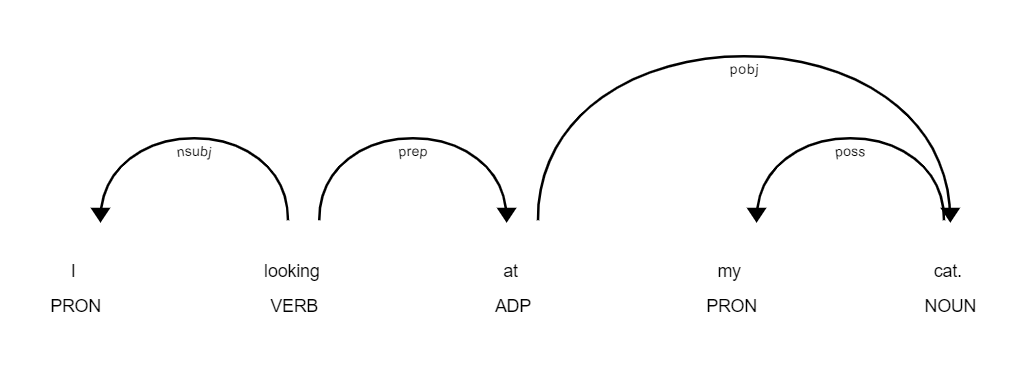
\includegraphics[scale=0.3]{depen.png}
		\end{figure}
	\end{frame}

	\begin{frame}[t]{Lemmatization}
		\textbf{Lemmatization} is the process of reducing inflected forms of a word while still ensuring that the reduced form belongs to the language. This reduced form or root word is called a lemma.\\
		
		example:
		
		is --> be\\
		looking --> look\\
		analytics --> analytic
	\end{frame}

	\begin{frame}[t]{Named Entity Recognition (NER)}
		A named entity is a “real-world object” that’s assigned a name – for example, a person, a country, a product or a book title.
	\end{frame}

	\begin{frame}[t]{Text Classification}
		Assigning categories or labels to a whole document, or parts of a document.
		\begin{figure}
			\centering
			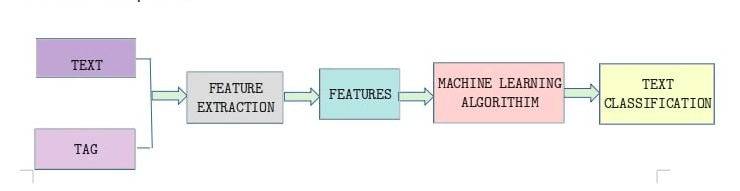
\includegraphics[scale=0.4]{text-classification-python-spacy.png}
		\end{figure}
	\end{frame}

	\begin{frame}[t]{What is Knowledge Graph?}
		\textcolor{OliveGreen}{A knowledge graph is a way of storing data that resulted from an information extraction task.} Many basic implementations of knowledge graphs make use of a concept we call triple, that is a set of three items(a subject, a predicate and an object) that we can use to store information about something.
	\end{frame}

	\begin{frame}[standout]
		Code
	\end{frame}
\end{document}